\chapter{Variable gear-ratio actuation technology}
\label{sec:MultipleSpeedActuationTechnology}

\section{Requirements}
\label{sec:Requirements}

\begin{figure}[H]
	\centering
		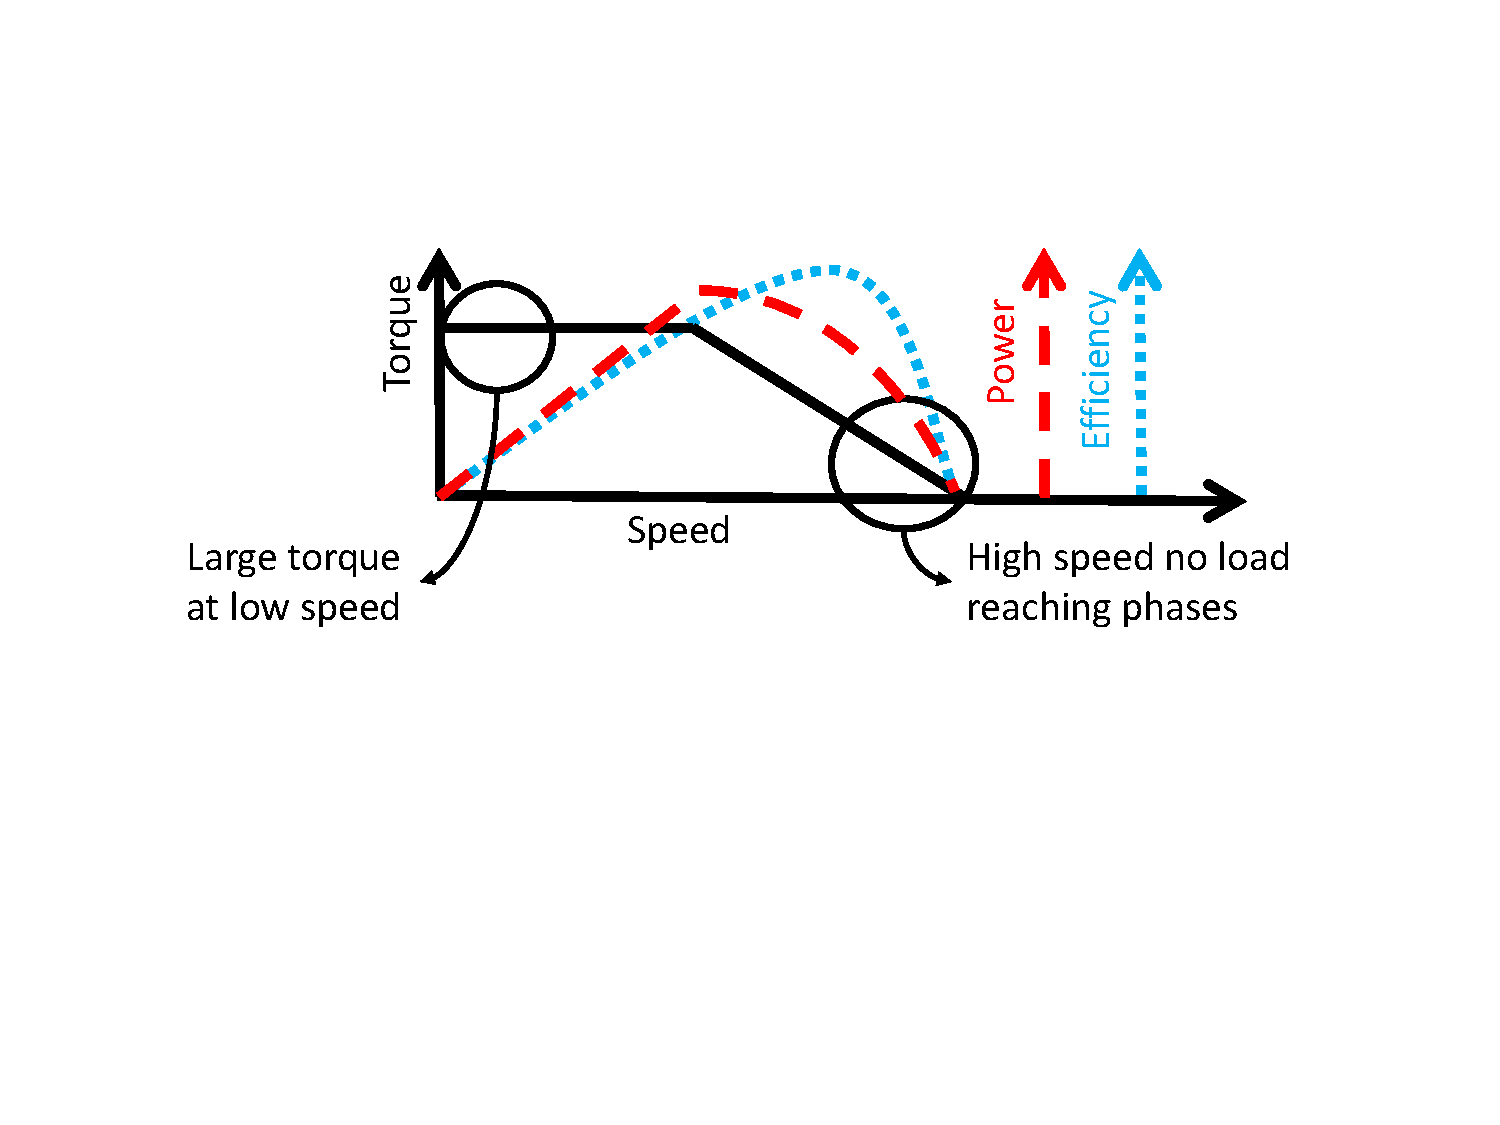
\includegraphics[width=0.45\textwidth]{speedissue.pdf}
	\caption{Limitations of EM motors for extremum torque-speed operations}
	\label{fig:speedissue}
\end{figure}


\section{Dual-Speed Dual-Motor architecture}
\label{sec:DSDM}


\begin{figure}[H]
	\centering
		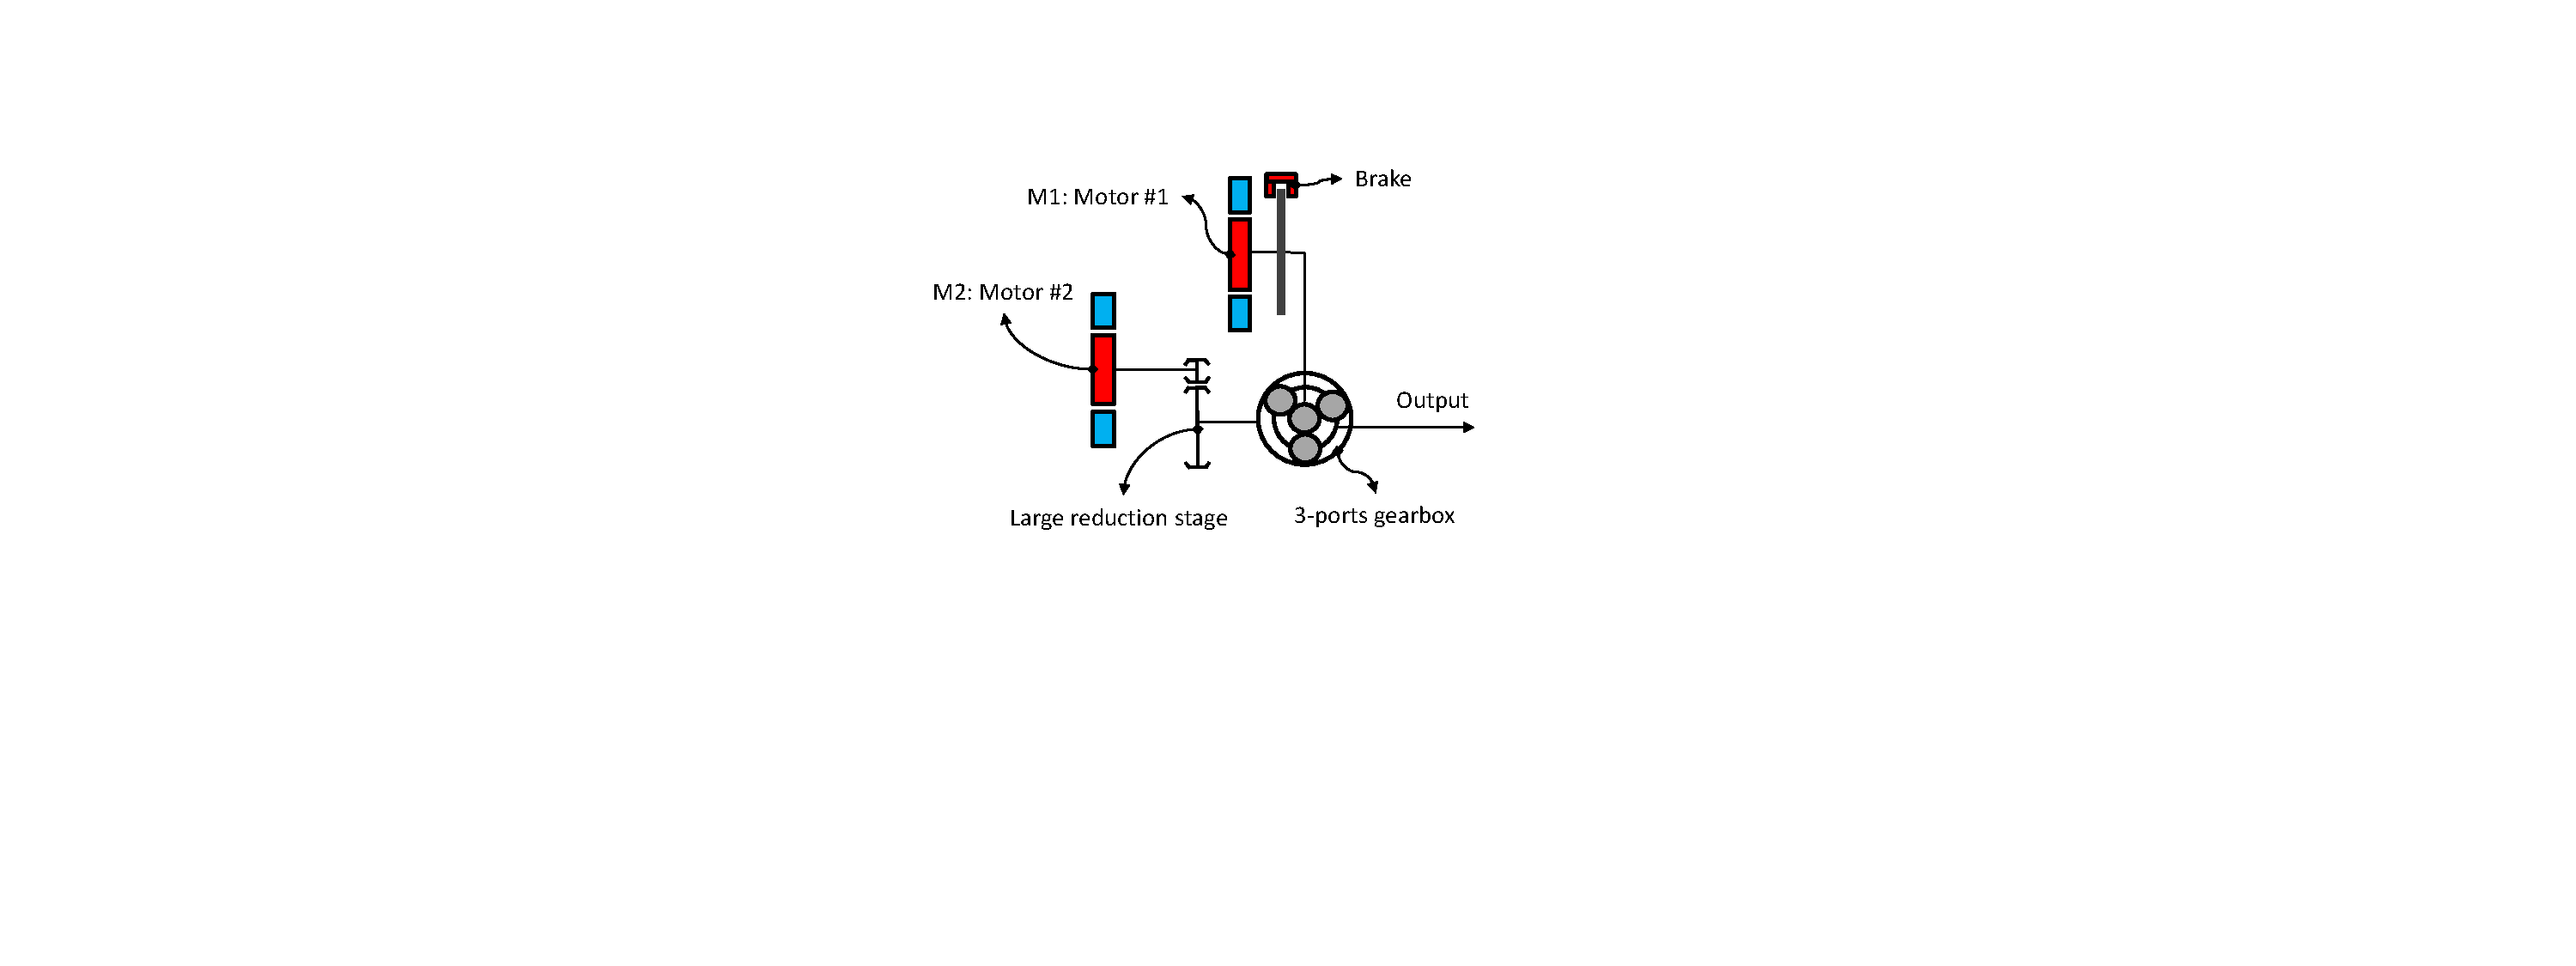
\includegraphics[width=0.40\textwidth]{dualmotorconcept2.pdf}
	\caption{DSDM actuator concept}
	\label{fig:dualmotorconcept}
\end{figure}


\begin{figure}[H]
	\centering
		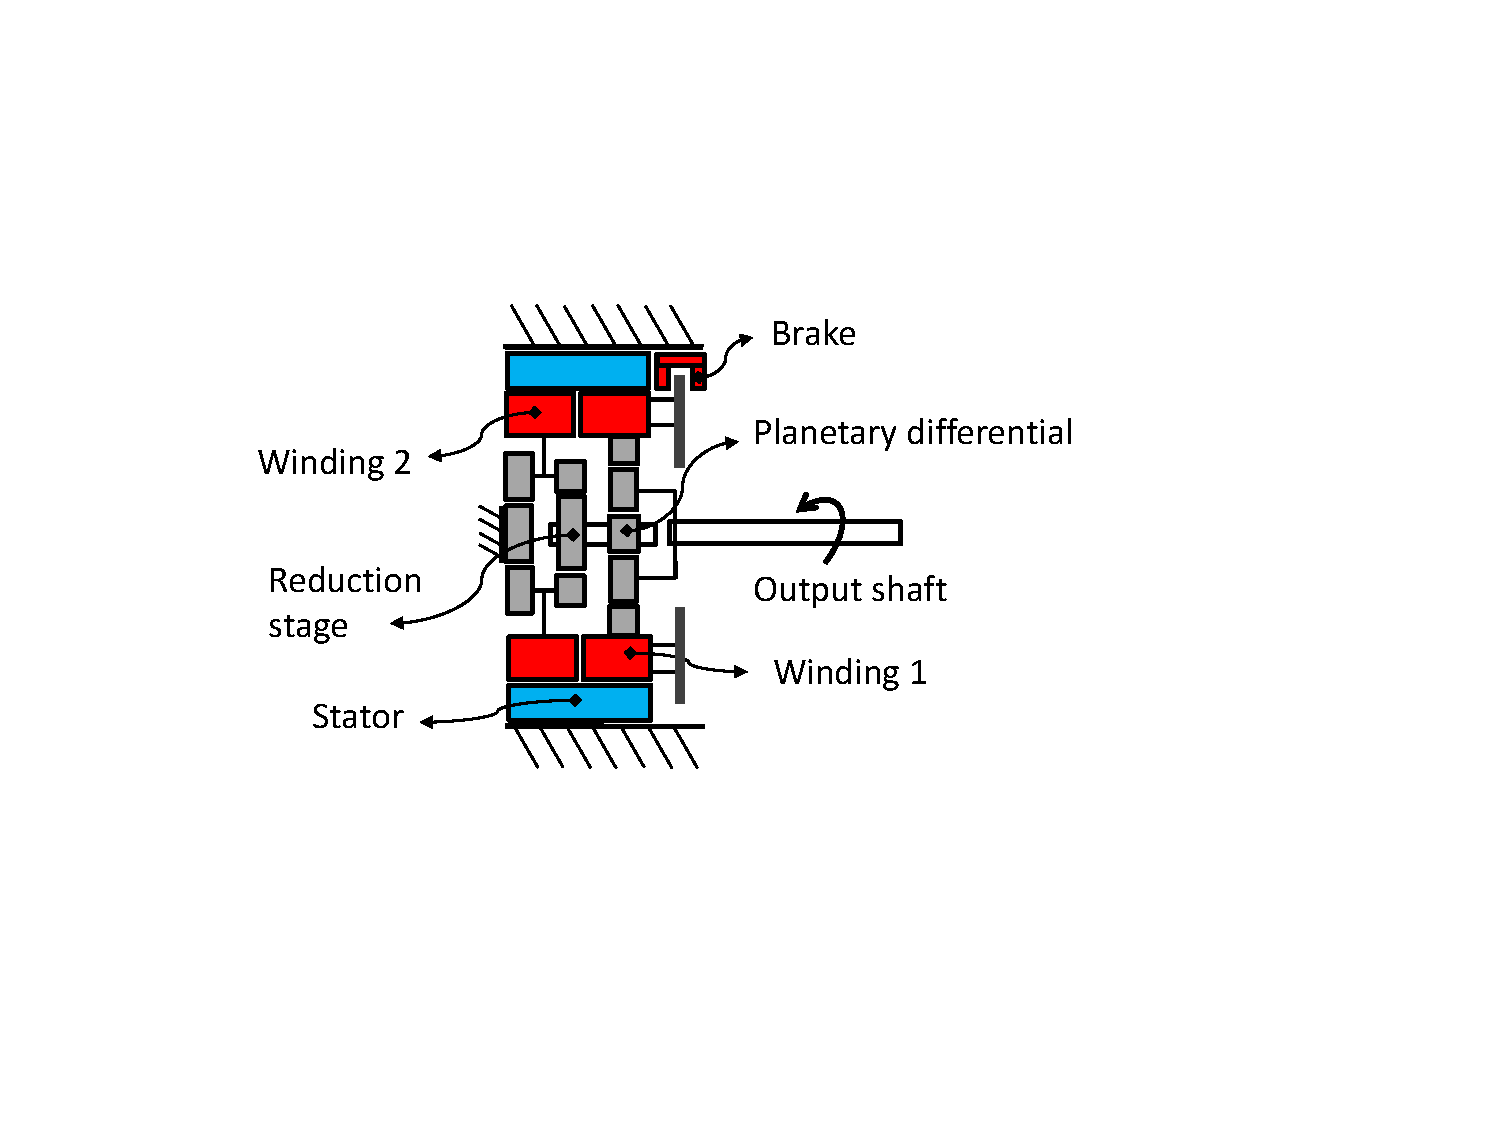
\includegraphics[width=0.40\textwidth]{embedded3.pdf}
	\caption{Possible architecture of an integrated DSDM concept}
	\label{fig:embedded}
\end{figure}


\begin{figure}[H]
	\centering
		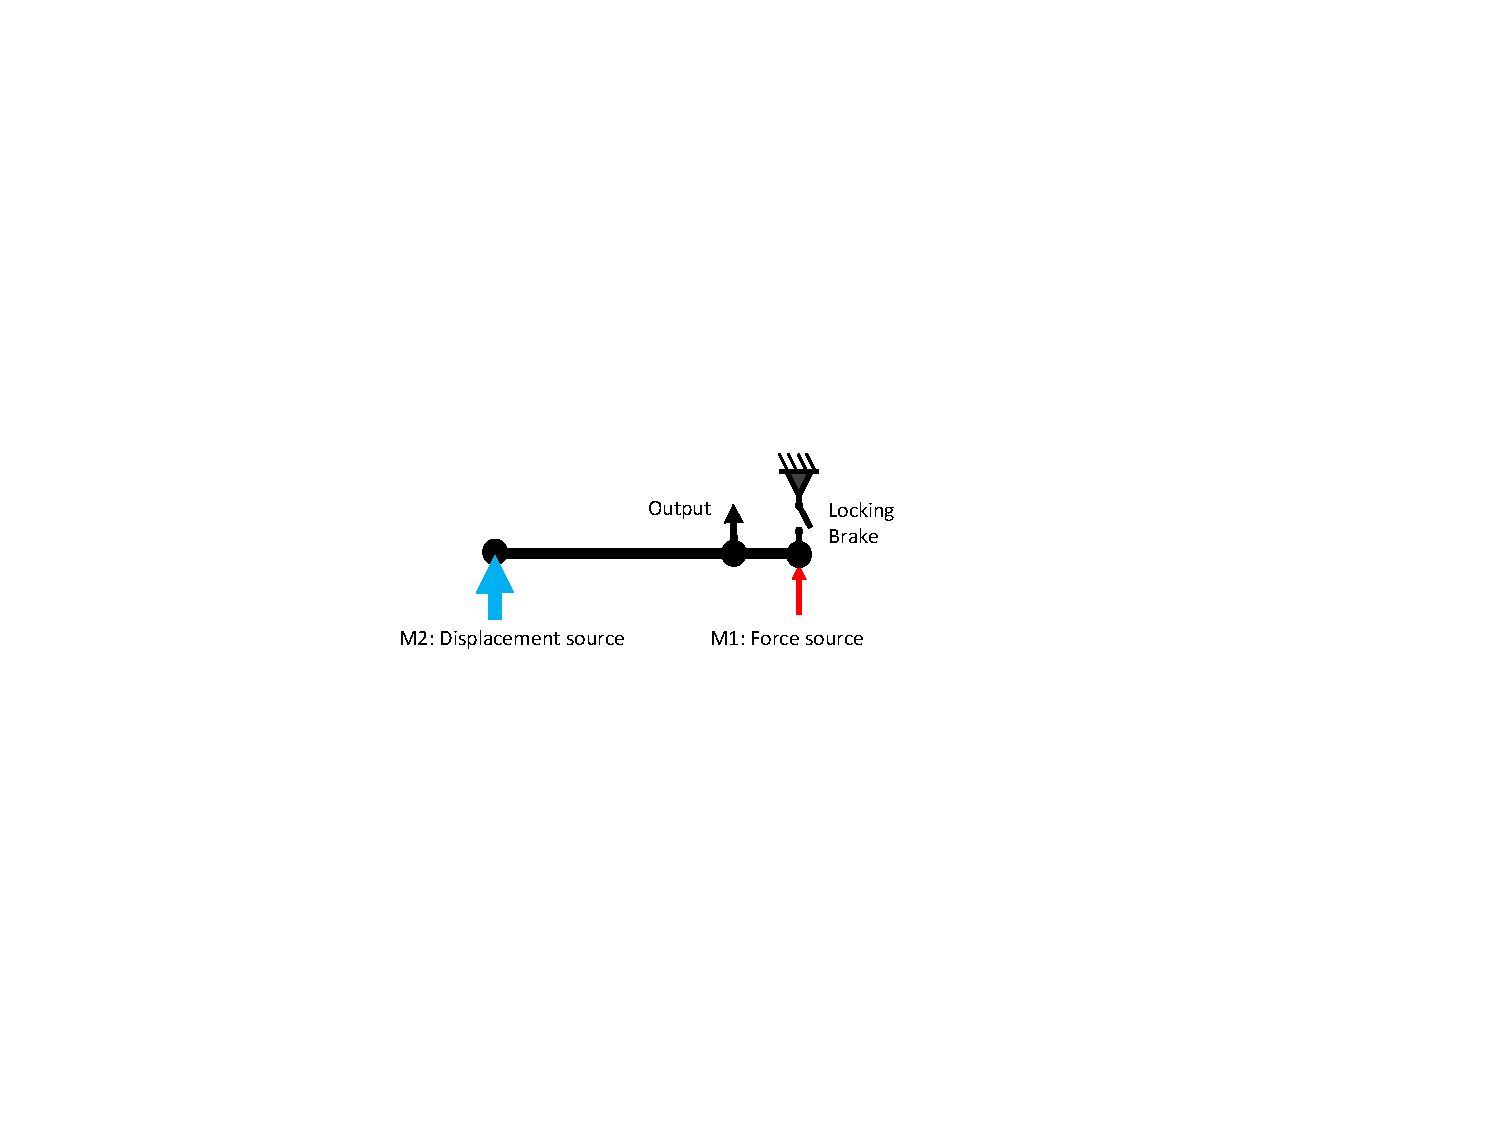
\includegraphics[width=0.40\textwidth]{lever.pdf}
	\caption{Dual input system}
	\label{fig:lever}
\end{figure}
%
\begin{figure}[H]
        \centering
				\subfloat[High force mode (brake closed)]{
        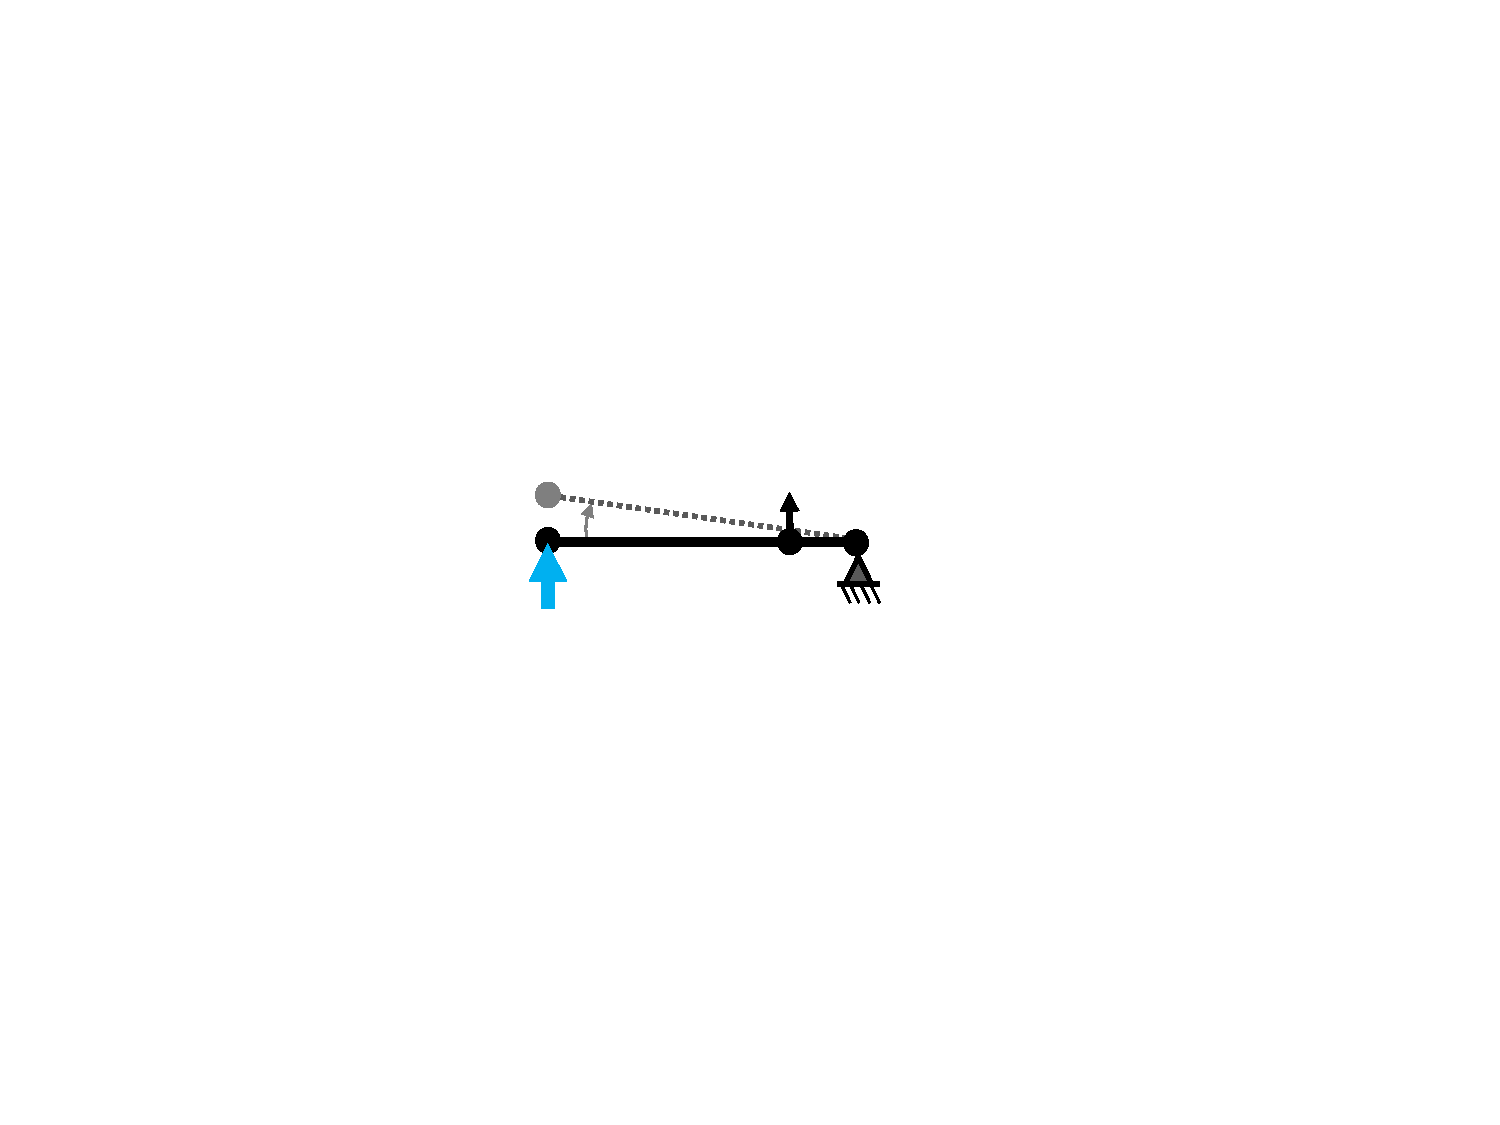
\includegraphics[width=0.22\textwidth]{leverHF.pdf}
				\label{fig:HF}}
        \subfloat[High speed mode (brake open)]{
				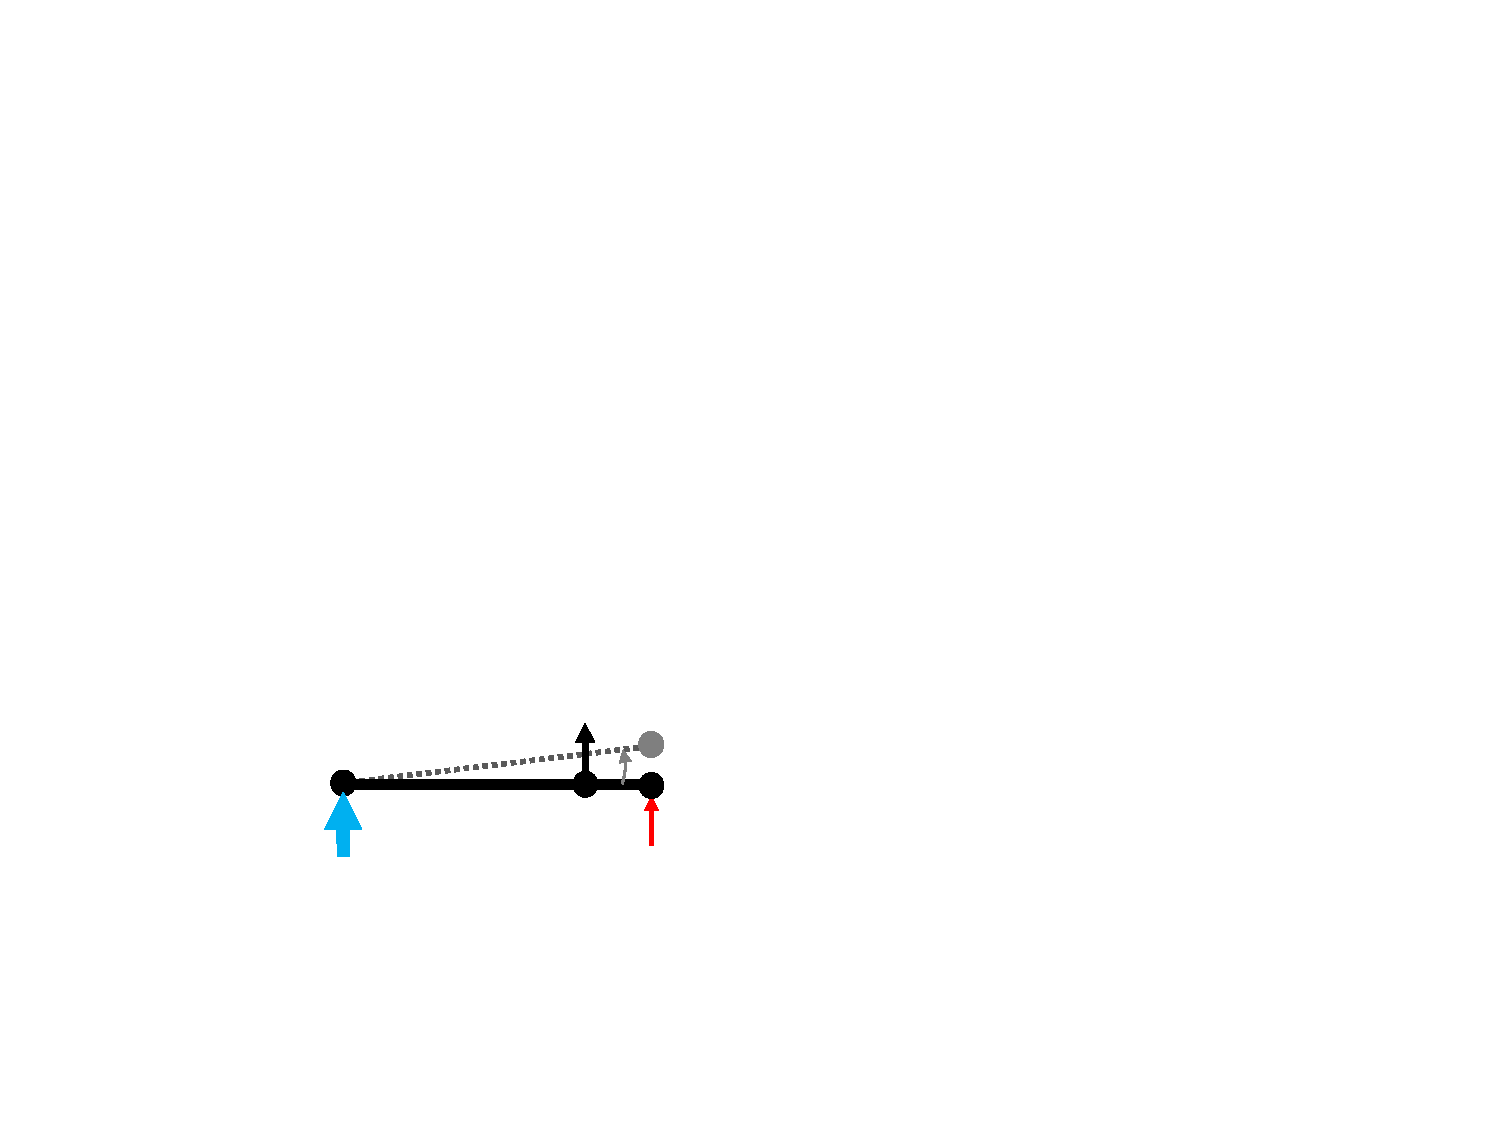
\includegraphics[width=0.22\textwidth]{leverHS.pdf}
				\label{fig:HS}}
        \caption{Two modes of operation}\label{fig:opmode}
\end{figure}

\begin{figure}[H]
	\centering
		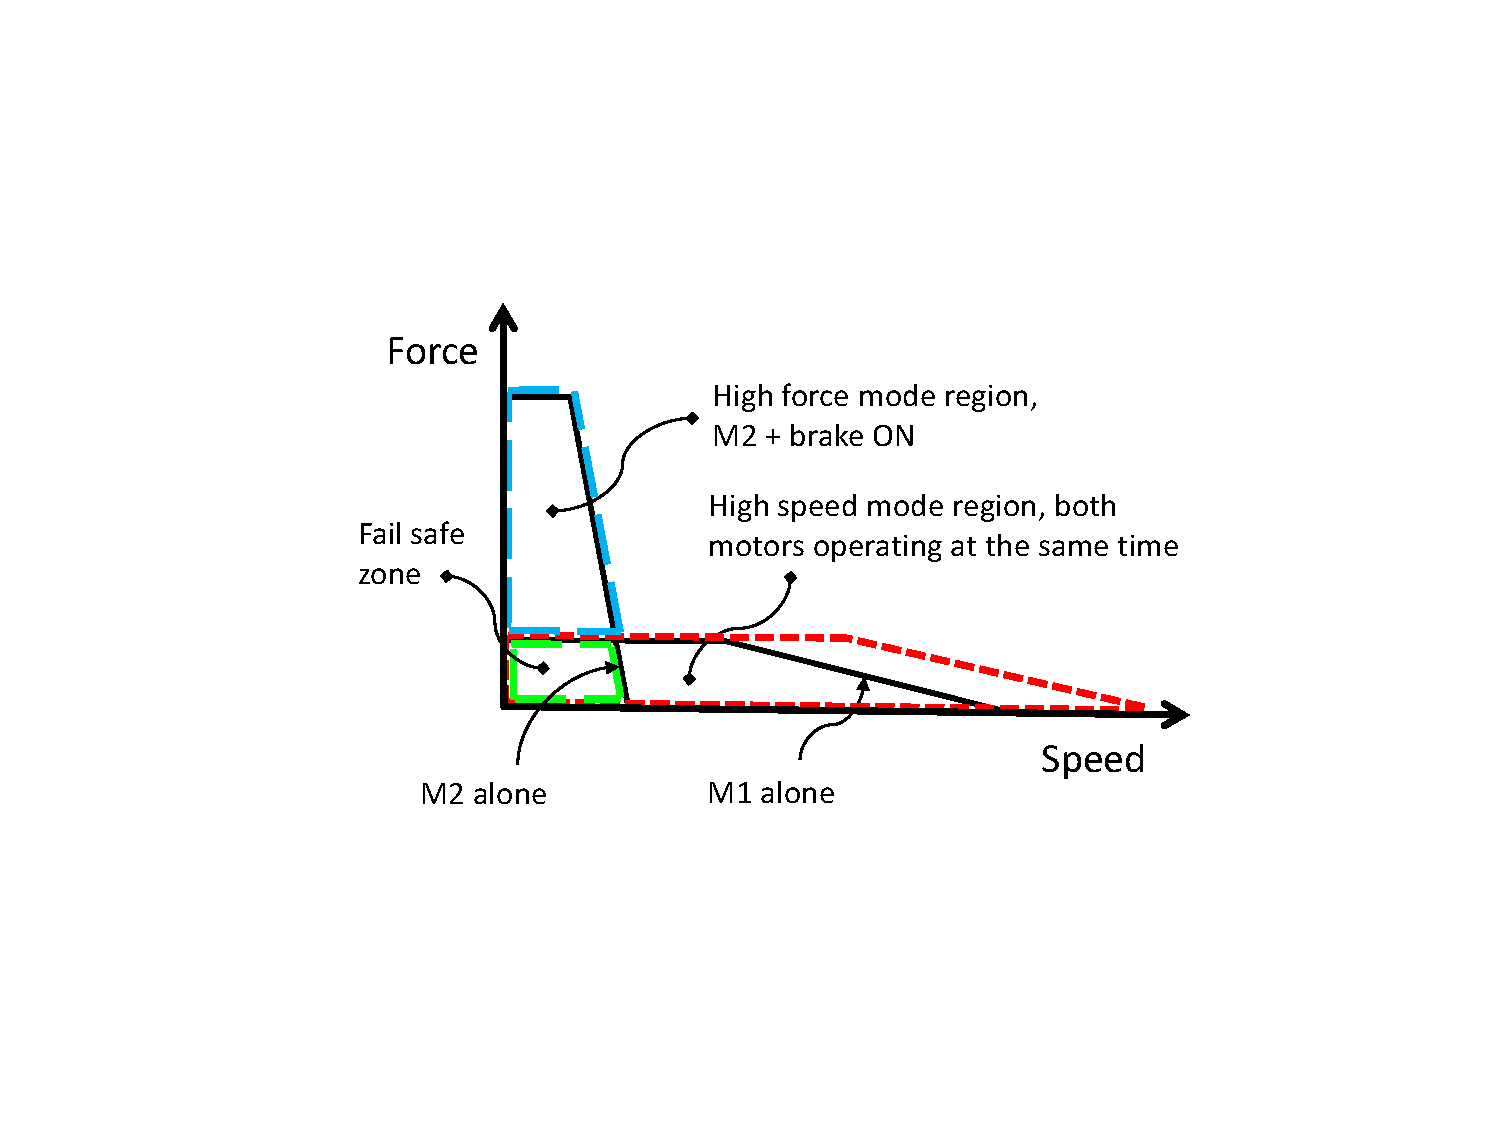
\includegraphics[width=0.45\textwidth]{torquespeed.pdf}
	\caption{DSDM actuator operation region, with a difference between M1 and M2 gearing ratio of only 4 for illustration purposes }
	\label{fig:torquespeed}
\end{figure}


\begin{figure}[H]
        \centering
				\subfloat[One motor solution]{
				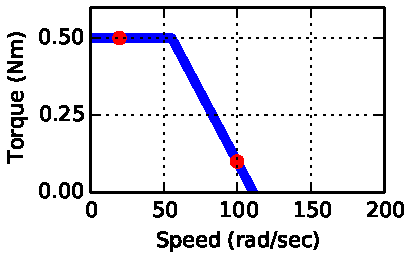
\includegraphics[width=0.22\textwidth]{sol1.pdf}
				\label{fig:s1}}
        \subfloat[DSDM solution]{
				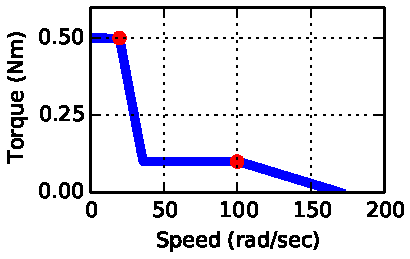
\includegraphics[width=0.22\textwidth]{sol2.pdf}
				\label{fig:s2}}
        \caption{Case study of two actuator solution for two 10 W operating points }\label{fig:solutions}
\end{figure}

\begin{figure}[H]
	\centering
		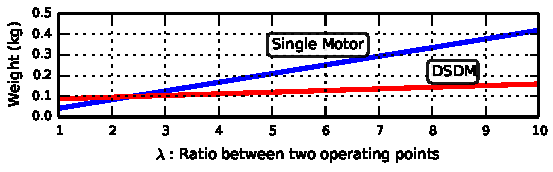
\includegraphics[width=0.45\textwidth]{w_vs_ratio.pdf}
	\caption{Weight of a single motor compared to the DSDM concept for two 10 W operating points at different speeds $w_1=100$ rad/sec, $w_2 = w_1 / \lambda$}
	\label{fig:1vs2}
\end{figure}


\section{Fast and Seamless gearshifts}
\label{sec:FastAndSeamlessGearshifts}

\begin{figure}[H]
	\centering
		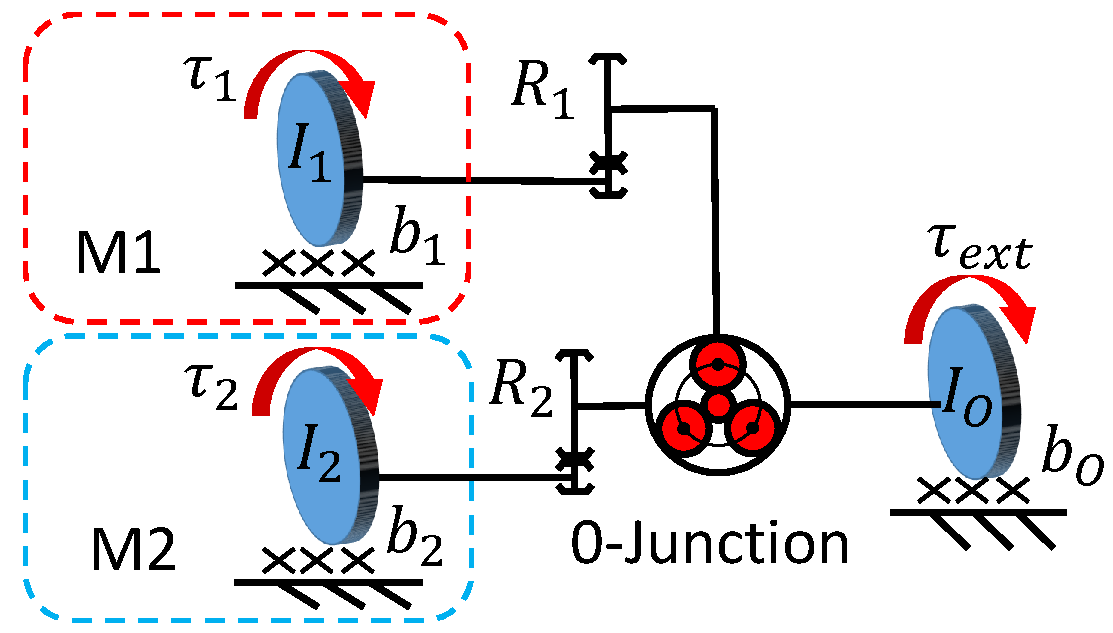
\includegraphics[width=0.45\textwidth]{dynamics.pdf}
	\caption{Lumped-parameter dynamic model of a DSDM}
	\label{fig:dynamics}
\end{figure}

\begin{figure}[H]
	\centering
		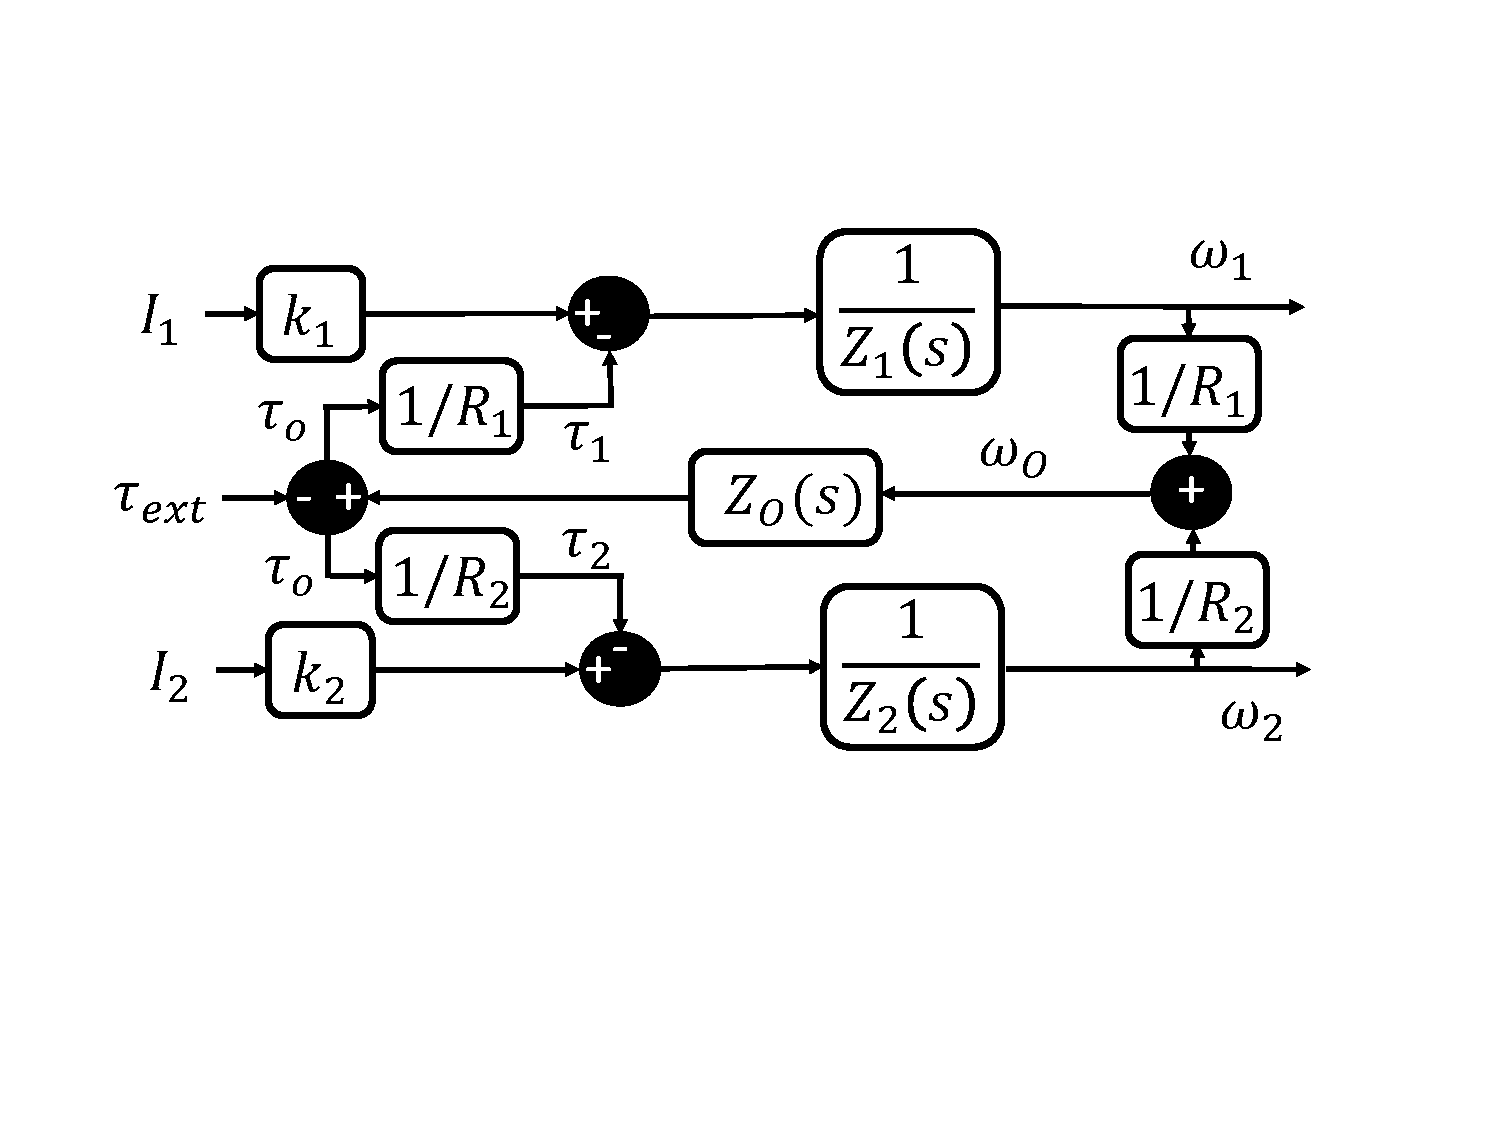
\includegraphics[width=0.40\textwidth]{dynamics_block.pdf}
	\caption{Dynamics of a DSDM}
	\label{fig:dynamics_block}
\end{figure}

\subsection{Nullspace of the system}

\subsection{Control Algorithm}


\begin{figure}[H]
	\centering
		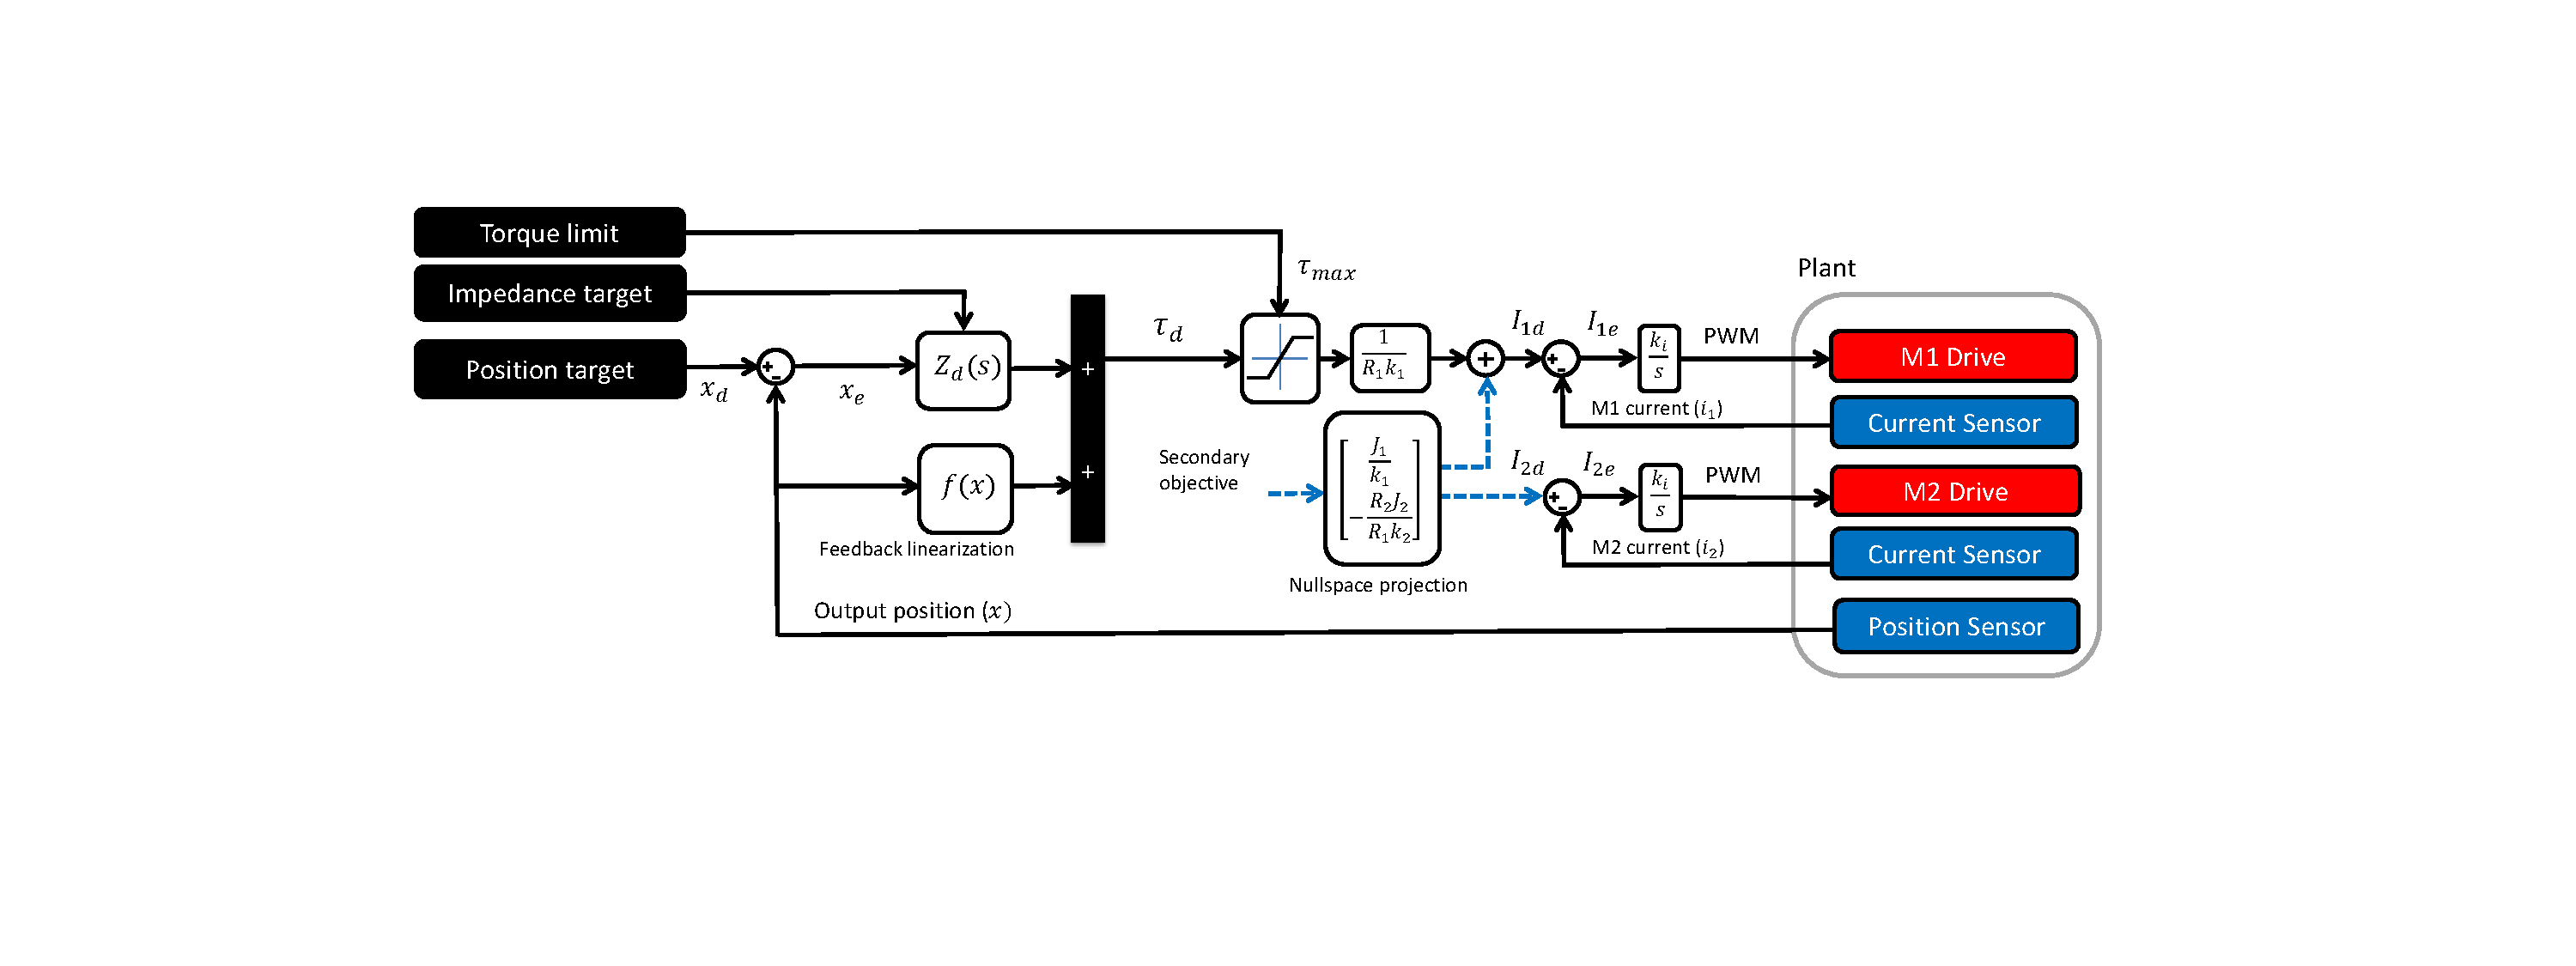
\includegraphics[width=1.00\textwidth]{HS_loop.pdf}
	\caption{High-speed mode control loop}
	\label{fig:HS_loop}
\end{figure}

\begin{figure}[H]
	\centering
		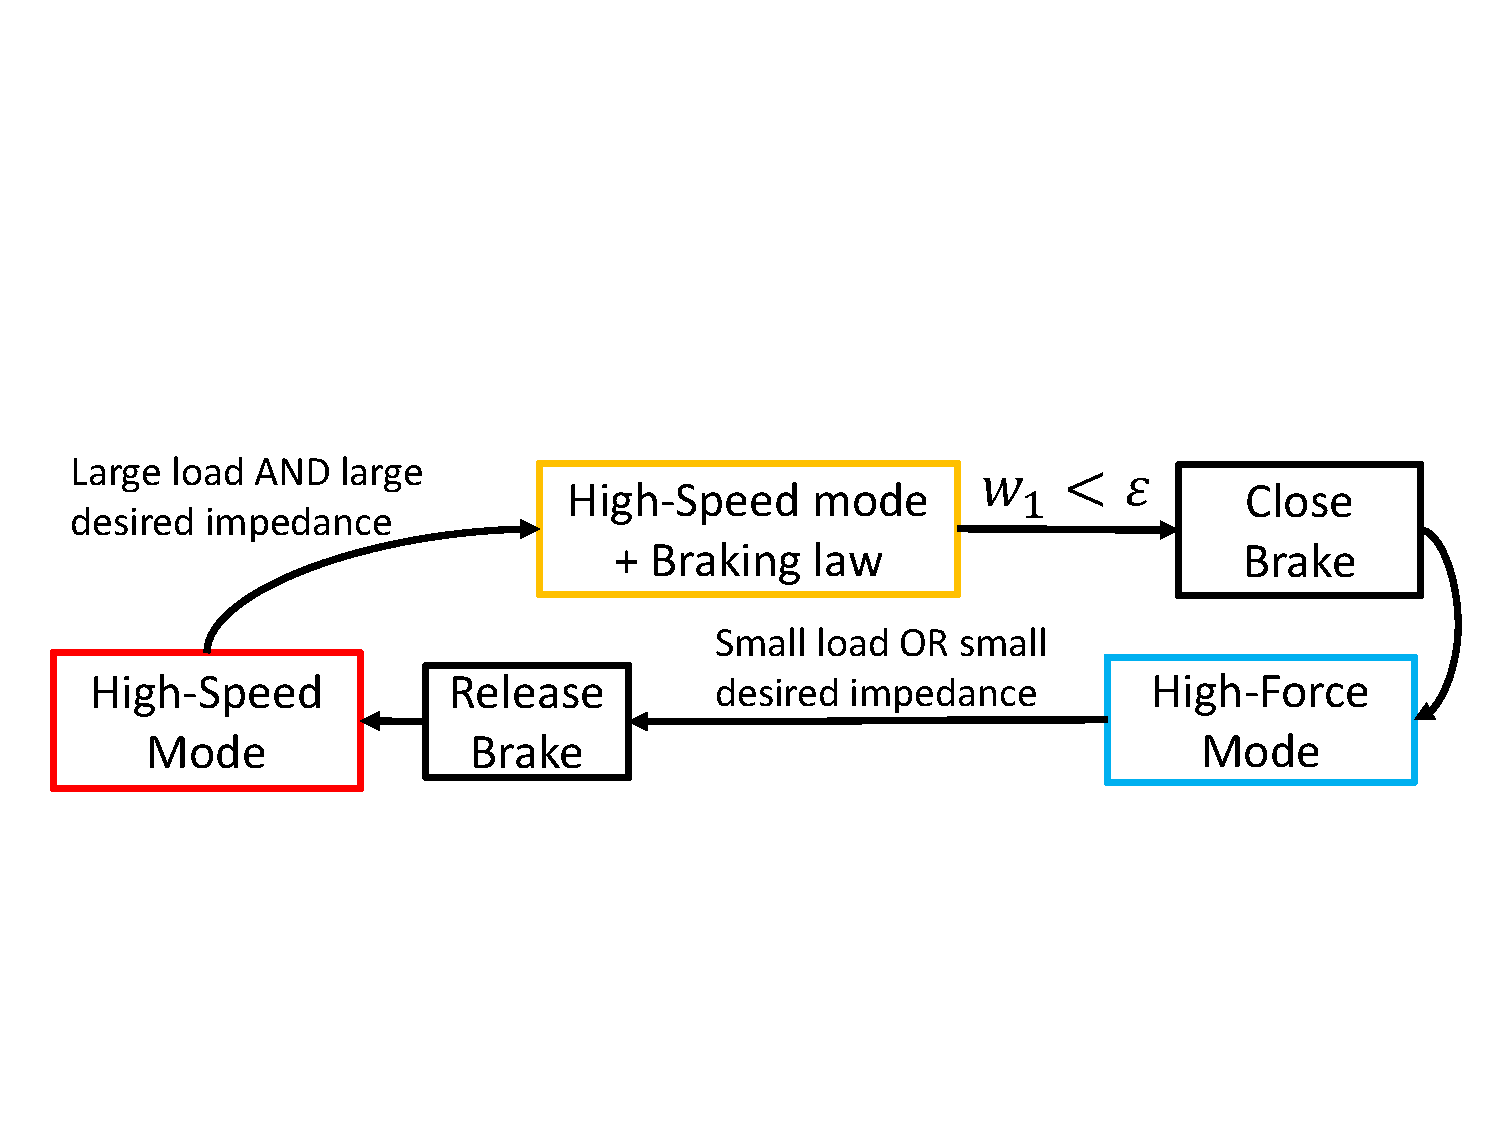
\includegraphics[width=0.45\textwidth]{automatic_flow.pdf}
	\caption{State machine for automatic mode selection}
	\label{fig:automaticflow}
\end{figure}

\section{Case studies for walking robots}
\label{sec:walking}



